\section{Unit test for CAN 4.4 used in Naiad}
\label{CAN_unit}
Unit test for the generic can card fitted in Naiad. \textbf{This test only test the basic electronics.} To fully test the card it is required to program it with a JTAG adapter and some kind of programming environment. The JTAG adapter is connected in to the analog-IO list on the left edge and are configured according to fig. \ref{JTAG}. This document can be used also in order to understand the card and below there is a list over what the LEDs in the bottom right corner mean.

\begin{figure}[!ht]
	\begin{center}
		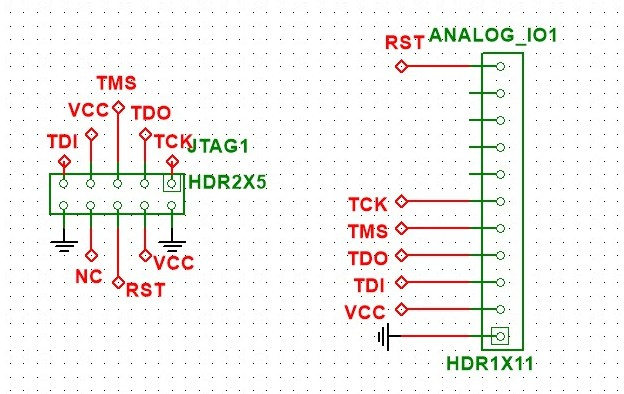
\includegraphics[width=0.76\textwidth]{./Images/Unit-Test-CAN/JTAG.jpg}
		\caption{The JTAG adapted needed to program the card.}
		\label{JTAG}
	\end{center}
\end{figure}

The card is divided in to three galvanically isolated fields. The fields are marked in fig. \ref{CAN_sections}. One for the processor and peripheral electronics (marked red), one for the CAN bus (marked green) and one for power Input (marked yellow). The two yellow field are connected on the back. 

\begin{figure}[!ht]
	\begin{center}
		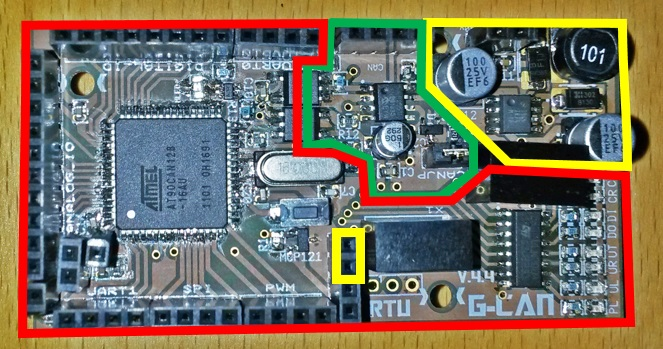
\includegraphics[width=0.76\textwidth]{./Images/Unit-Test-CAN/CAN_sections.jpg}
		\caption{The CAN cards different fields marked, the fields are galvanic isolated}
		\label{CAN_sections}
	\end{center}
\end{figure}

\noindent In the lower right corner there are a list of LEDs the silk screen can be quite cryptic here is a explanation. 

\begin{itemize}
\item CT = CAN Transceiver, light up when a CAN message in sent
\item CR = CAN Receive, light up when a CAN message in received
\item DI = TDI, has to do with the JTAG, lights up when the card is being programmed
\item DO = TDO, has to do with the JTAG, lights up when the card is being programmed
\item UR = UART Transceiver, light up when a UART message in sent
\item UR = UART Receive, light up when a UART message in sent received
\item UL = User LED, programmable LED that can be set by setting leg 6 on the processor. (In version 5 (also called motor CAN) this LED has been moved to pin 14)
\item PL = Power LED should light up as soon as power is turned on
\end{itemize}

\subsection {Required resources}
\begin{itemize}
\item Card for testing
\item Power supply, 12-48V
\item Multi-meter
\end{itemize}


\newpage
\subsection{Input}
The input consists of some protective circuitry and a switched regulator that takes the input and switches it down to 12 V. Connect the input voltage (12.6-48V) to the break way header on the top right corner. Ground is the left connector. 

\begin{figure}[!ht]
	\begin{center}
		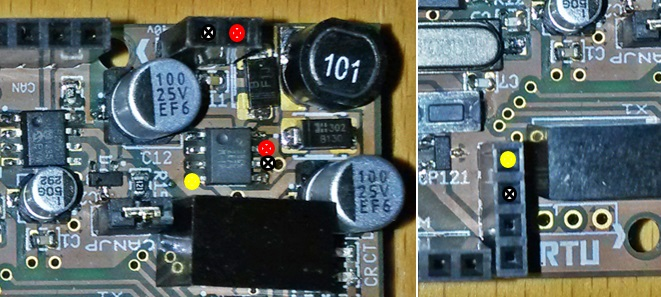
\includegraphics[width=0.76\textwidth]{./Images/Unit-Test-CAN/CAN_input.jpg}
		%\caption{The caption you want with the picture}
		\label{CAN_input}
	\end{center}
\end{figure}

\begin{table}[ht]
\begin{tabularx}{\textwidth}{|c|>{\hsize=0.6\hsize}X|>{\hsize=0.6\hsize}X|c|>{\hsize=1.8\hsize}X|} %>{\hsize=.5\hsize}X>
\hline 
Point/Net & Pre-condition: & Desired & Measured & Commentary \\ 
\hline 
GND &  & 0V / 0$\Omega$ &   & Check that the GND on the card and supply are the same  \\ 
\hline 
Input & Supply with 12.6-48V & Input voltage 12.6-48V  &    & As soon as the supply is connected the bottom LED in the bottom right corner should light up. If does not there is some errors on the card. Make sure the supply is correct. Then check the inputs to the DC-DC (the two middle legs on the right side) \\ 
\hline 
Output & Supply voltage & 12V &   & Measure between the same black as above and the yellow dot. If there is no output here it is most likely the DC-DC that’s broken try to change that.  Measure also in the breakaway header in the lower middle part of the card. If there is 12 V up in the corner and not here there is a problem with the traces on the back \\  
\hline
\end{tabularx}
\end{table}

\newpage
\subsection{CAN power}
\begin{figure}[!ht]
	\begin{center}
		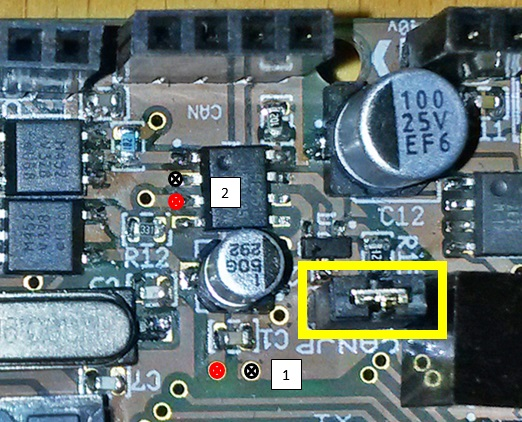
\includegraphics[width=0.76\textwidth]{./Images/Unit-Test-CAN/CAN_power.jpg}
		%\caption{The caption you want with the picture}
		\label{CAN_power}
	\end{center}
\end{figure}

\begin{table}[ht]
\begin{tabularx}{\textwidth}{|c|>{\hsize=0.6\hsize}X|>{\hsize=0.6\hsize}X|c|>{\hsize=1.8\hsize}X|} %>{\hsize=.5\hsize}X>
\hline 
Point/Net & Pre-condition: & Desired & Measured & Commentary \\ 
\hline 
Can VCC & Supply voltage & 5V &   & If there is no power between the dots (1) there is either the trace from the DC-DC or the DC-DC \textbf{below} (not in picture) that is broken. Check the traces and then try to replace the DC-DC \\ 
\hline 
Supply for CAN & Supply voltage & 5V  &    & Check that the CAN circuit get its required input (2) \\ 
\hline 
Jumper & - & - &   & It is not necessary to have jumper on all nodes but it is preferred. (marked yellow) \\  
\hline
\end{tabularx}
\end{table}

\newpage
\subsection{Processor with peripherals}
The rest of the cards and the 5V output for shields are driven by the DC-DC marked in the picture in yellow.
\begin{figure}[!ht]
	\begin{center}
		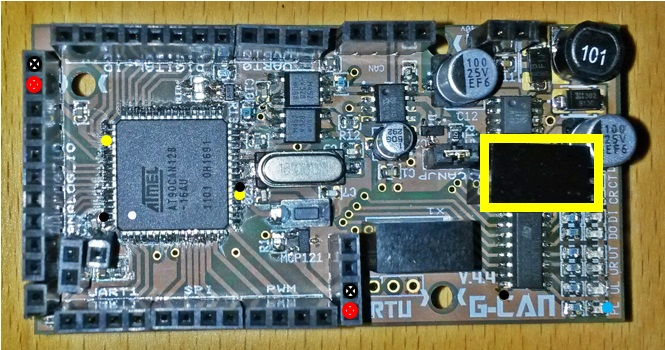
\includegraphics[width=0.76\textwidth]{./Images/Unit-Test-CAN/CAN_processor.jpg}
		%\caption{The caption you want with the picture}
		\label{CAN_processor}
	\end{center}
\end{figure}

\begin{table}[ht]
\begin{tabularx}{\textwidth}{|>{\hsize=0.6\hsize}X|>{\hsize=0.8\hsize}X|>{\hsize=0.8\hsize}X|c|>{\hsize=1.8\hsize}X|} %>{\hsize=.5\hsize}X>
\hline 
Point/Net & Pre-condition: & Desired & Measured & Commentary \\ 
\hline 
VCC & Supply voltage & 5V &   & Measure both big red/back dots. If none are 5V measure leg 3 and 4 on the yellow marked DC-DC (3 is GND), replace if incorrect voltage here to. If one of the pair is 5V and not the other there is a broken trace somewhere.\\ 
\hline 
Power LED & Supply voltage & LED on / 5V  &    & The LED on the bottom in the bottom left corner should light up. If it doesn’t check that the voltage between the blue dot and the closest small black dot is 5V. If so the LED or resistor is probably broken, try to change these. If not the trace between the LED and the DC-DC is probably broken. \\ 
\hline 
Supply for MCU & Supply voltage & 5V &   & Measure the small yellow and black dot located on the processor. (2$^{nd}$ from the bottom and 3$^{rd}$ from the top on the left and 5$^{th}$ and 6$^{th}$ from the bottom on the right) \\  
\hline
\end{tabularx}
\end{table}

\newpage

